%===================================== CHAP 5 =================================

\chapter{Implementation}\label{ch5:implementation}

To be able to answer the research questions using the methods described in the previous chapter, a system needed to be developed. This chapter covers the implementation and architecture of this system and its different components, including decisions on design, usability and development.

\section{System overview}

Utsida contains two sub-systems, where the first part is a web application, and the second part is a case-based reasoning recommender system (CBR-RS). Each part primarily focuses on one of the research questions. The web application is designed to increase the motivation (RQ1), while the CBR-RS finds out how suitable CBR is to give recommendations on exchange universities and courses (RQ2). The recommendations made by the CBR-RS could also affect the motivation (RQ1). Utsida was chosen as the name of the system due to being a counter opposite to NTNU's central system \emph{Innsida}, and the meaning of the word \emph{inside}. Utsida gives a relation to something on the outside, in this case going on an exchange program. The requirements identified in the preliminary research (sec \ref{sec:requirements})  was used as the basis for the choices made on design and implementation.

As illustrated by Figure \ref{fig:system_overview}, the web application part communicates with the CBR-RS part. Queries are sent from the web application by a user and received by the CBR-RS through its REST\footnote{Representational State Transfer} API\footnote{Application Programming Interface}. These queries are in turn matched against the entire case-base in the CBR-RS. Finally, all the cases are given a similarity score based on the user query and then returned to the web application. Typically in a CBR system, the solution to a problem would be the solution of the case with the highest similarity score for the proposed problem. Utsida, on the other hand, offers several possible solutions because it uses a case-based \textbf{recommender} system, rather than a case-based \textbf{reasoning} system. This way, the user can see several solutions, and pick the one they want.  

\begin{figure}[H]
    \centering
    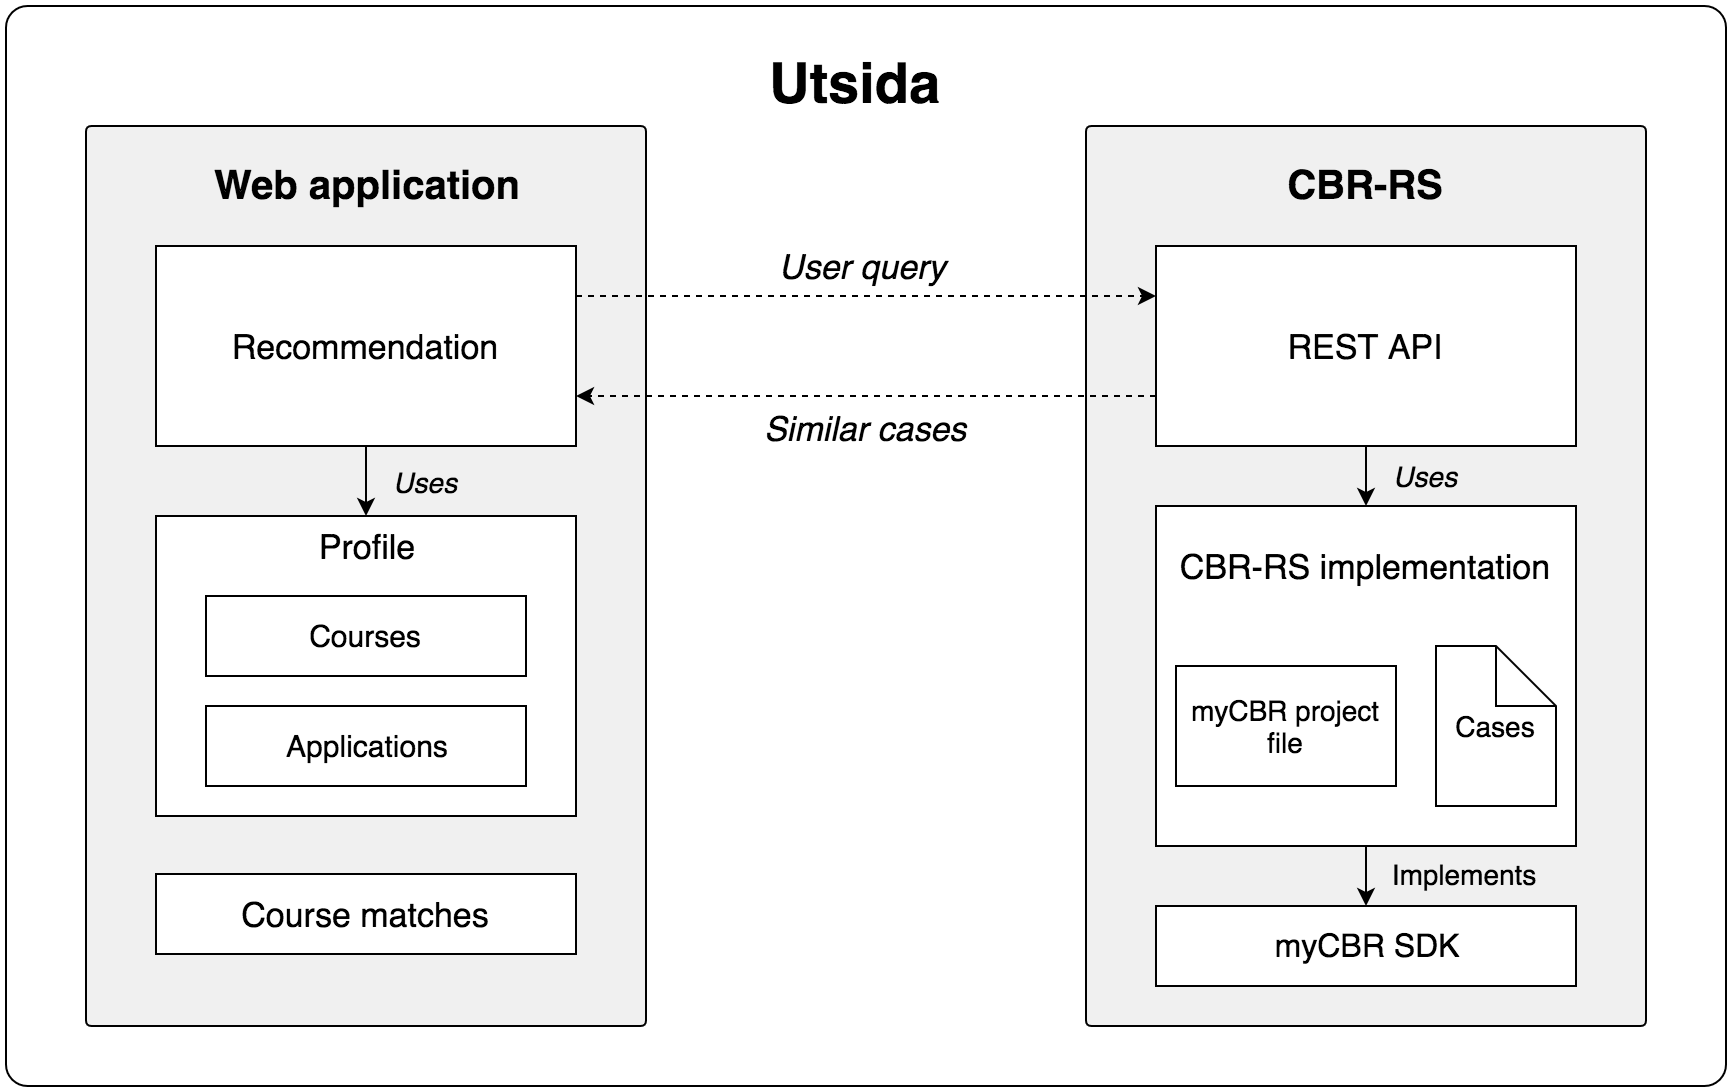
\includegraphics[width=1\textwidth]{fig/system_overview.png}
    \caption{Abstract architectural diagram of Utsida}
    \label{fig:system_overview}
\end{figure}

\section{Data and Information}

Utsida requires up to date organizational data about NTNU to be usable. This includes all the courses, faculties and departments at NTNU. This data was gathered with IDI's organizational API\footnote{http://www.ime.ntnu.no/api/}. This API is, however, discontinued, so to update this data after 2016, a new data source would have to be found. Furthermore, the course matches component (sec. \ref{sec_course_matches}) in the web application relies on information on previously approved course matches\footnote{Sets of courses where one or more courses from another university are approved by advisers as a replacement for a course at NTNU}. To avoid a cold start, some approved course matches from IDI were parsed and used in the component. The most critical data, however, was the data used to create cases for the CBR-RS, namely the \textit{experience reports}. All the data was analyzed according to the six primary dimensions for data quality assessment\cite{askham2013six} to gain awareness of the possible limitations before deciding on Utsida's database model.

\subsection{The Experience Reports}\label{sec:experience_reports}
Most students who go on an exchange program from NTNU has to write obligatory reports about their exchange experience to the OIR, called experience reports. These reports are available to the public, and are written in the period between 1999 and 2016. Because they include a large amount of information on exchange experiences, they proved to work as a great foundation for the cases. Typically, the case-base in a CBR-RS is start of with a low amount of cases and gradually expand as new cases are retained. In this project, however, it was essential to have an initially large number of cases. Therefore, all of the current public experience reports were parsed and used as cases in the CBR-RS' case-base. 

\subsection{Parsing the Experience Reports}\label{sec:parsing_experience_reports}

The experience reports are essentially large text files in HTML\footnote{Hypertext Markup Language} format. To be able to use them in the CBR-RS, all the useful information in the files had to be extracted and parsed to cases in a CSV file, which is the file format used for case-bases in myCBR. This was done with a custom script written in the Python programming language. In short, all available experience reports (HTML files) were first downloaded and stored in a directory. Next, the script looped through all the HTML files, read the internal data with the HTMLParser\footnote{https://docs.python.org/2/library/htmlparser.html} Python package, and finally stored all the useful data in a CSV file. This way, each row in the CSV file would correspond to one case with the attributes given by Table \ref{tab:case_representation2}. This process resulted in a CSV file with 8702 cases which formed the case-base used in the CBR-RS.

A large part of fields in the experience reports were free text, which means that the format of each field was decided by the report author and did follow any standard. The parsing script, therefore, had to use specific methods to parse each attribute to the correct format. Two methods were primarily used to parse the data; data dictionary look-ups and approximate string matching, also called fuzzy searching. Edge cases that were not detected by these techniques were solved with basic string operations. In the end, most of the data in the experience reports was transformed into usable data in the CBR-RS. It was, however, not possible to make sure that 100\% of the data in the experience reports were parsed to a correct format while still keeping its original meaning.

\paragraph{Fuzzy Searching}

Fuzzy Searching is an algorithm used to recognize patterns and similarities in a text. To determine the similarity, it yields a similarity score between two textual inputs. By using this technique in the parser script, the data in the experience reports could be mapped against a predefined set of attributes, and return the attribute which are most similar to the input data. For example, the department field in the experience reports had a significant variation of abbreviations and ways of spelling. By creating a dictionary with all departments and faculties, fuzzy searching could be used to find the department in the dictionary with the highest similarity to the department in the experience report. This is illustrated in Figure \ref{fig:fuzzy_searching}. This method was also used on the university field to avoid creating multiple instances in the database. Several more Python dictionaries were configured to be able to map the necessary data in the experience reports to a correct format. These includes dictionaries for countries, continents, languages, universities, departments, and faculties.

\begin{figure}[h]
    \centering
    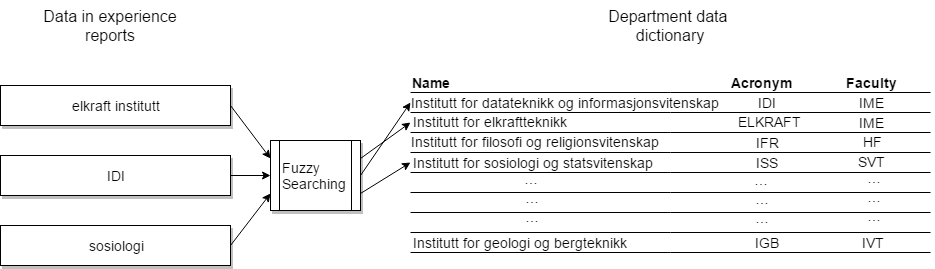
\includegraphics[width=1.0\textwidth]{fig/fuzzy_search.png}
    \caption{Input data is transformed to a set format by using fuzzy searching}
    \label{fig:fuzzy_searching}
\end{figure}

\section{The Web Application}

This section presents the different components of the web application, used tools and frameworks and reasoning for design and usability choices.

\subsection{Components}

The web application part of Utsida is divided into three main components, as Figure \ref{fig:system_overview} depicts; \emph{Recommendations, Profile} and \emph{Course matches}. The goal of the components as a whole is to answer RQ1 and to increase the motivation of students to go on an exchange program. Each component targets one or several of the requirements of Utsida, listed in Table \ref{tab:feature_list} The requirements are referenced in a REQ\# format, with \# as the requirement number. REQ5 is handled by the web application in the index page and not by any component.

\subsubsection{Recommendation}

The recommendation component target REQ1 of the Utsida system, and is used to answer RQ2. This component handles all the communication with the CBR-RS part; Queries made by users are sent in the JavaScript Object Notation (JSON) format to the CBR-RS through HTTP requests, which returns all of its cases and their respective similarity score, also in JSON format. In this component, a user can select their preferences and requirements for an exchange program (see Figure \ref{fig:web_results_1} and \ref{fig:web_results_2}). The user is then presented with a list of the best suiting universities for their query. The universities in the list can each be selected to show the best matching experiences for that university. Each experience contains a list of courses taken, and serves as a recommendation.

\subsubsection{Course Matches}\label{sec_course_matches}

The course matches component target REQ2 of the Utsida system, and its purpose is to display all approved course matches that are stored in the web application. The component filters course matches by which university they are approved for, and supports adding, deleting, commenting and editing of course matches by student advisers. For a student, this component serves as a resource where they can search and find replacements for their courses at NTNU, get information about the courses and the approval of them, and save the course match to their profile.

\subsubsection{Profile}

The profile component handles all user related functionality, such as authentication, and contains the required personal information about each student. The personal information includes the user's current department at NTNU, which the web application use in a recommendation query. The component has two sub-components: Courses and Applications.

\paragraph{Courses} 
is a sub-component of the profile component and targets REQ3. It contains functionalities which enables a student to organize their application process. This includes storing courses at home, courses abroad and course matches. From the course page (see Figure \ref{fig:web_courses}) students can also manually match abroad- and home courses to create new course matches for their applications. This component serves as a large part of the whole course match approval process and is essential for the digitalization of the process.

\paragraph{Applications} 
is another sub-component of the profile component and targets REQ4. It stores course approval applications submitted by users. Where the application contains the course matches a user wants to get approved by a student advisor. It also maintains the functionality needed to create applications. For students and student advisers, the application component serves as a digital version of the current paper-based application system where student advisers can approve, reject, and remove students' applications, while students can easily keep track of them. This component is an extension needed to complete Utsida as possible replacement of NTNU's current approach.

\begin{figure}[h]
    \centering
    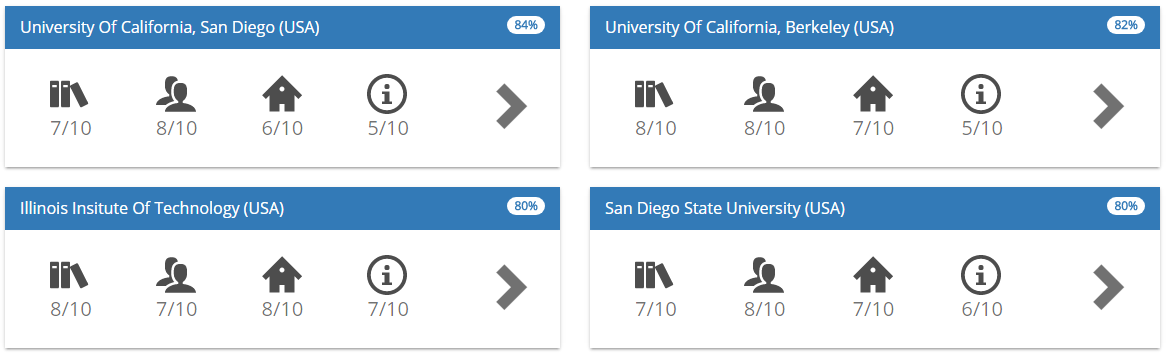
\includegraphics[width=1\textwidth]{fig/utsida_screenshots/results_1_cut.png}
    \caption{How results are first presented after sending a query in Utsida}
    \label{fig:web_results_1}
\end{figure}

\begin{figure}[h]
    \centering
    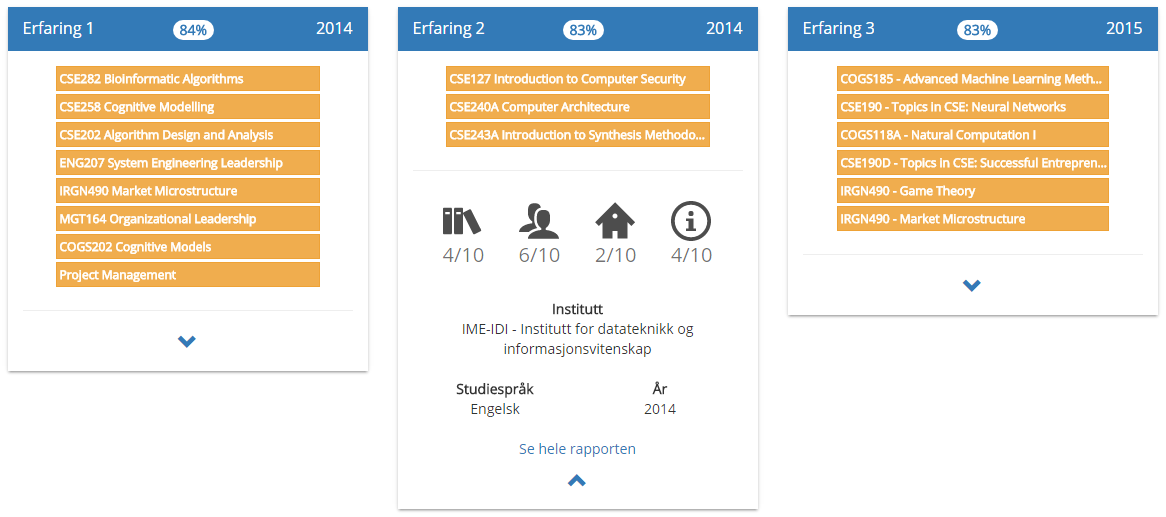
\includegraphics[width=1\textwidth]{fig/utsida_screenshots/results_2_cut.png}
    \caption{How results are presented after selecting a recommended university in Utsida}
    \label{fig:web_results_2}
\end{figure}

\begin{figure}[H]
    \centering
    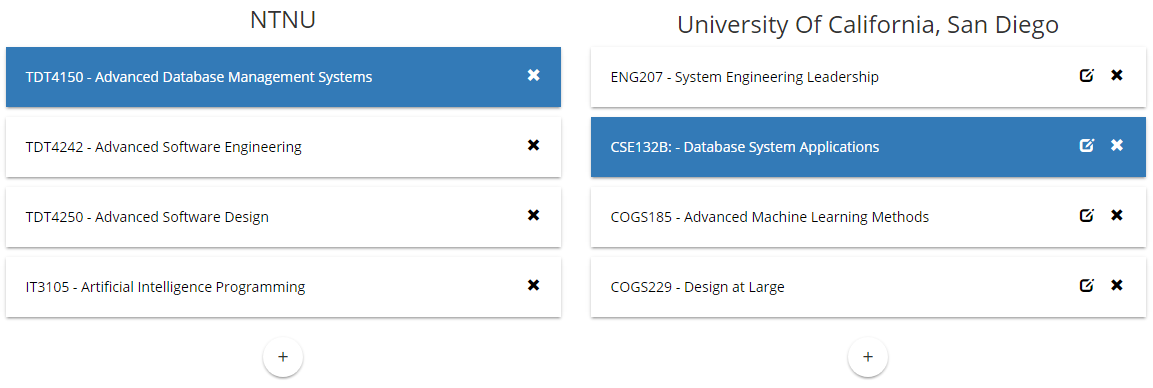
\includegraphics[width=1\textwidth]{fig/utsida_screenshots/course_match_cut.png}
    \caption{The view for saving, viewing and matching courses in Utsida.}
    \label{fig:web_courses}
\end{figure}

\subsection{Tools and frameworks}
When developing the web application part of Utsida, several tools and packages were used to simplify the development process and to acquire functionality which would not be feasible to develop from scratch. Django (sec \ref{sec:django}) was chosen as the main web framework.

To enforce a responsive and aesthetic design, Bootstrap 3\footnote{http://getbootstrap.com/} was used as a front-end Cascading Style Sheets (CSS) framework. jQuery\footnote{https://jquery.com/} was used as a front-end JavaScript framework to simplify HTTP requests, which this system largely relies on both internally in the web application and between the web application and the CBR-RS. A collection of packages for the Python language was also used. These packages include Fuzzywuzzy\footnote{https://pypi.python.org/pypi/fuzzywuzzy}: a packages which handles apprximate string matching, Requests\footnote{http://docs.python-requests.org/en/master/}: a package for writing HTTP requests from Python, and Python-social-auth\footnote{https://python-social-auth.readthedocs.io/en/latest/} combined with Dataporten-auth\footnote{https://pypi.python.org/pypi/dataporten-auth/0.1} to enable using authentication methods such as Feide, the authentication service used at NTNU.

\paragraph{Django}\label{sec:django}

Django\footnote{https://docs.djangoproject.com/en/1.11/}, a web framework using the Python programming language, was chosen as the web framework to develop the web application in. Django is maintained by the Django Software Foundation (DSF). The DSF calls it an MTV-framework, meaning \emph{Model, Template, View}, which in practice functions as a Model View Controller (MVC) pattern. Django includes many built-in features such as a SQLite database, a predefined directory structure, controllers to handle communication between the different components, and several others. Another important feature is Django's built-in security packages, which handles security risks such as Cross-Site Request Forgery, authorization and Cross-site scripting. Django also includes an administrator panel, which enables management of database models with a simple interface. In conclusion, the reason for choosing Django as the main framework was because it offered a complete package that reduced time used on structural difficulties and made it possible to focus on the usability and evaluation methods.

\subsection{Design \& Usability}

The design in terms of both functionality and aesthetics was an integral part of the development of the web application part of Utsida. Questionnaires were used as the main data collection method to gather data on how Utsida performed in terms of motivational effect as well as evaluation of the validity of the system's recommendations. This was all conducted in a remote manner, which removes the option for the authors to help the test subjects with eventual issues. Therefore, the system had to be designed in a way which would produce as little issues and hardships for the users as possible, to make sure they understood how to use it, and thus were able to truly evaluate it.

The design of Utsida is inspired by the User Centered System Design-perspective, proposed by Norman \& Draper \cite{norman1986user}. Potential users of the system was included throughout the development process, either with small hallway tests, interviews, or usability tests. These tests let the users try out the system on their own, followed by questions as \enquote{How would you expect this functionality to work?}, \enquote{Was it easy to navigate the system?} and \enquote{Was it intuitive to understand how that functionality works?}. Several measures was implemented to strive for a user centered design, including:

\begin{itemize}
    \item Personalized items: Buttons and links to parts of the application which contains data which related to the user are prefixed with the word \emph{My}. For example, \emph{My courses, My profile, my applications.}
    \item Inline help text: Some parts of the application contain help text for those users that might need it. The help texts are shown by hovering over or clicking a question mark button. 
    \item Streamlined process: The process flow is displayed as a numerated process to guide the user, shown in Figure \ref{fig:utsida_index}.
\end{itemize}

\begin{figure}[h]
    \centering
    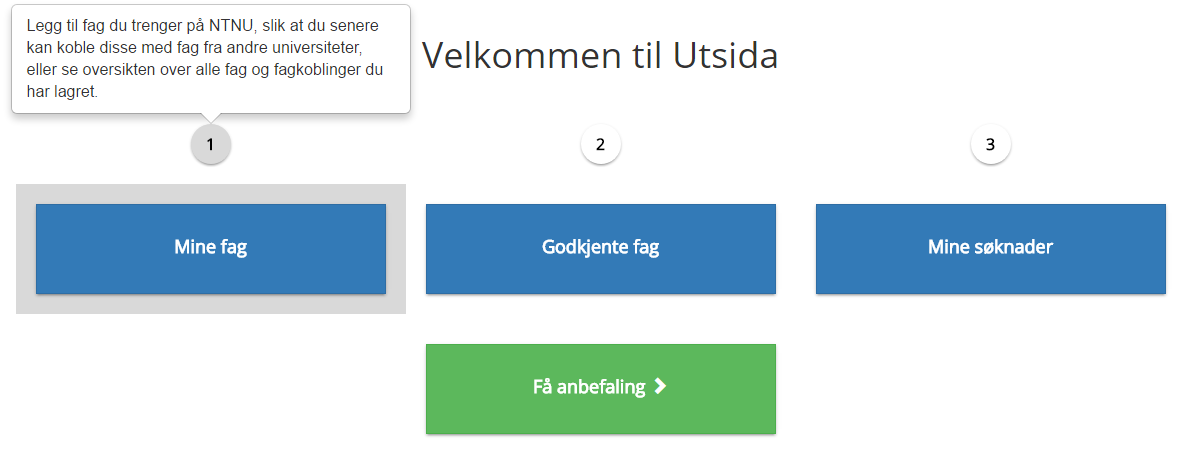
\includegraphics[width=1\textwidth]{fig/utsida_screenshots/steps.png}
    \caption{Index page of Utsida's web application}
    \label{fig:utsida_index}
\end{figure}

\section{The CBR-RS}

This section describes how the CBR-RS was modeled with the myCBR Workbench and how it was implemented to give the most relevant recommendations. Furthermore, it includes how the cases are represented, which similarity measures that are used, how the weighting of the attributes in the exchange experience concept was done, and how the system itself is structured.

\subsection{Overview}

The CBR-RS is a customized version of an open-source Java Spring\footnote{https://spring.io/} application that implements the myCBR SDK. To serve requests from a web application the Java application uses a REST API implemented with the Swagger API\footnote{http://swagger.io/}. This architecture made it possible to let both the web application and the CBR-RS be two independent systems, only communicating through HTTP\footnote{Hypertext Transfer Protocol} requests. The CBR-RS imports a custom myCBR project file which contains the case-representation, the similarity measures used on each attribute and the attributes' weight values. It also imports a CSV file used as the case-base, containing all of the cases.

When a request is made by a user in the web application, a query is first sent to the CBR-RS. When the CBR-RS receives the query it performs the first step of the CBR-cycle, by using the retrieve operation in the myCBR SDK. The exchange experiences are then ordered from highest to lowest similarity and finally the exchange experiences with the highest similarity scores are returned to the web application. Figure \ref{fig:retrieval_process_diagram} displays how a request made by a user in the web application traverse between the two systems to return a list of the most similar exchange experiences.

\begin{figure}[h]
    \centering
    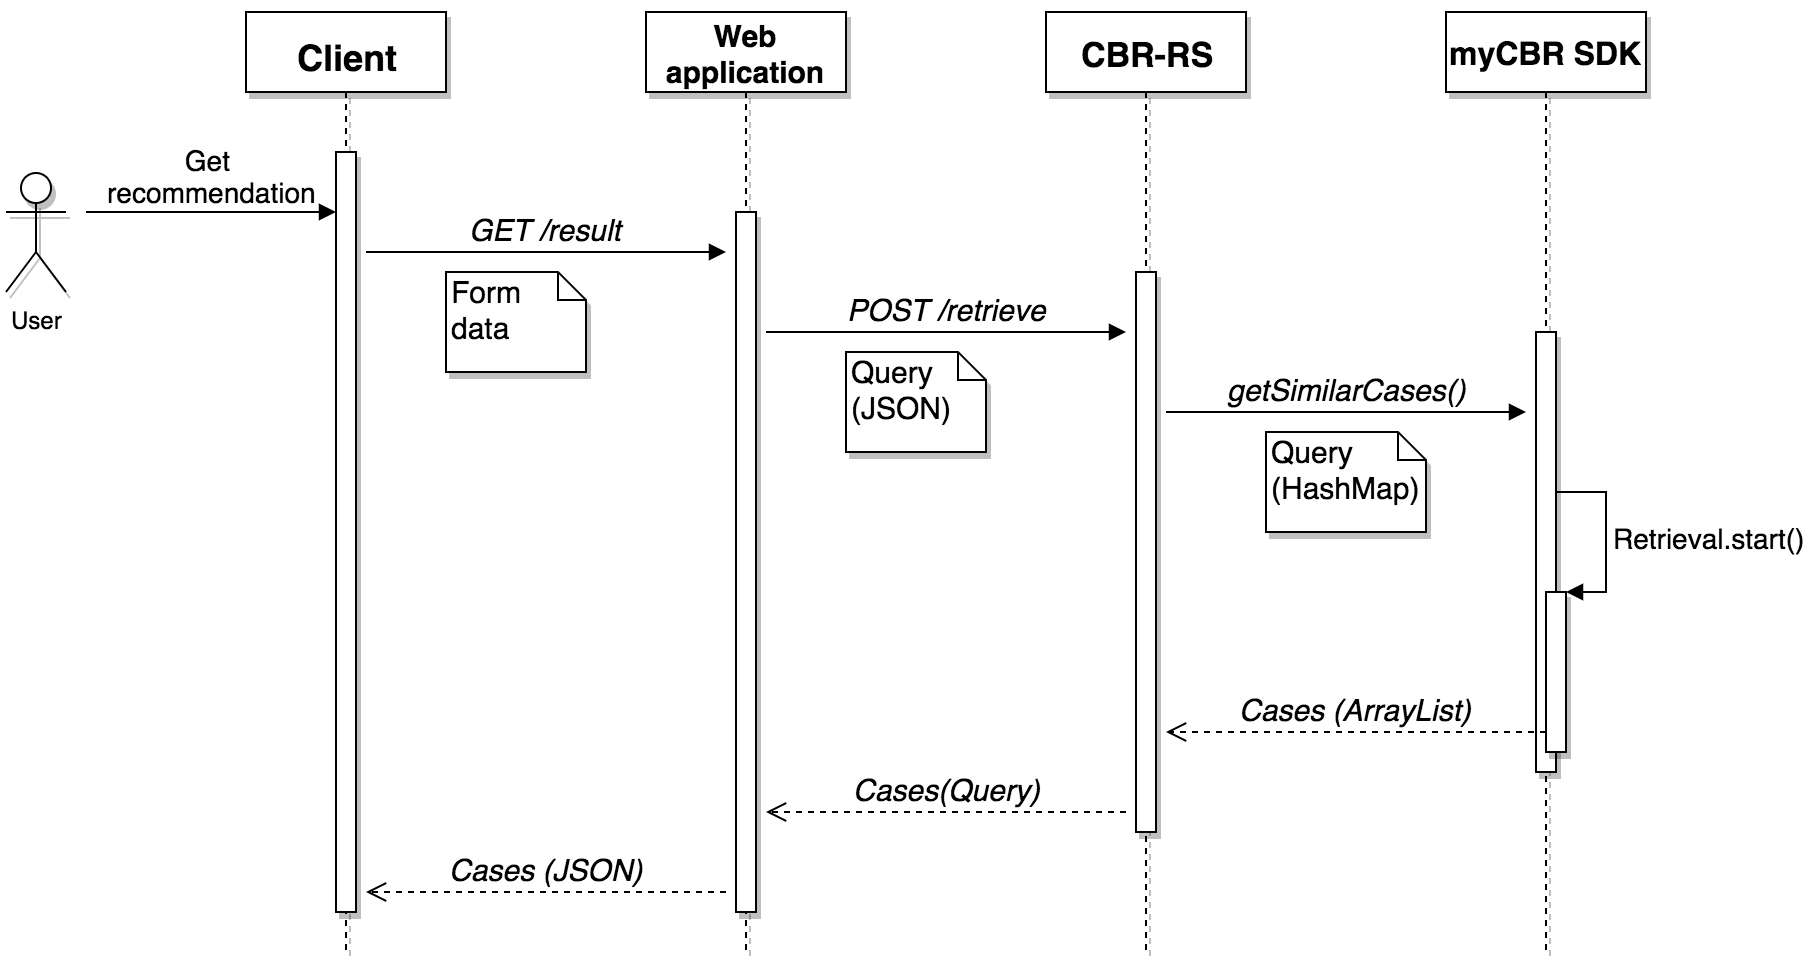
\includegraphics[width=1\textwidth]{fig/RetrievalProcessDiagram.png}
    \caption{Sequence diagram which shows how the initial user input is handled before returning as similar cases}
    \label{fig:retrieval_process_diagram}
\end{figure}

\subsection{Case Representation}

The exchange experience reports are the underlying data the CBR-RS use to give recommendations. These reports contains a large amount of data, and therefore not all of it is relevant. Only a small part of the data was used to ensure that Utsida gives relevant recommendations and is straightforward to use. The first choice of data to use for the initial case representation were based on personal experiences and a study by Cubillo et. al. (2006) \cite{maria2006international} that identified groups of important motivational factors. This representation was, however, extended in an iterative process of usability tests and then finalized by using the data collected from questionnaire 1 (sec \ref{sec:questionnaire_1}). The final case representation is displayed in Table \ref{tab:case_representation2}. 

\begin{table}[h]
\centering
\small
\caption{Final case representation in the CBR-RS}
\label{tab:case_representation2}
\begin{tabulary}{\textwidth}{|L|L|}
\hline
\textbf{Attributes} & \textbf{Example Case} \\ \hline \hline
Department & IME-IDI - Institutt for datateknikk og informasjonsvitenskap \\ \hline
Continent & North America \\ \hline
Country & USA \\ \hline
University & UCLA \\ \hline
Language & English \\ \hline
Study Period & 2012 \\ \hline
Academic Quality Rating & 8 \\ \hline
Social Quality Rating & 4 \\ \hline
Ease to find- and quality of residential & 5 \\ \hline
Support and reception at university & 6 \\ \hline
Subjects Taken & \begin{tabular}[c]{@{}l@{}}COMP1927 - Computing 2\\ MATH3220\\ CS4210\\ DATA101\end{tabular} \\ \hline
\end{tabulary}
\end{table}


\subsubsection{The Problem Part}

The problem part of a case is all the attributes which denotes a user's preferences, and profile information about them. The following list elaborates the choice and significance of the different attributes used in a case.

%Hva
%Hvorfor
%Hvordan

\begin{itemize}
\item \textbf{Department:} A profile attribute which details the department a user belongs to. It is considered the most important attribute, as it highly indicates what kind of courses (i.e. solution) which are relevant to a user. 

\item \textbf{Continent:} A preference attribute which implies which continent a user wish to travel to. Allows for a less precise location than a country.

\item \textbf{Country:} A preference attribute which implies which country a user wish to travel to. Serves as the most precise geographical location a user can select.

\item \textbf{University:} A preference attribute which lets a user include a specific university they wish to go to.

\item \textbf{Language:} A preference attribute which represents the study language the user wish to have.

\item \textbf{Study Period:} A hidden attribute which is the current year for a query. In a case, it implies the year an exchange experience was made. It is included to make older cases less relevant to the user, as university courses often change over time.

\item \textbf{Academic Quality Rating:} A preference attribute which combines an experience report's \emph{Academic Quality}, \emph{Special Competence Gained} and general \emph{Quality of Academic Opportunities}. Each of these aspects is related to the academic quality of an experience, and are weighted differently.

\item \textbf{Social Quality Rating:} A preference attribute which is a conjunction of an experience report's rating of  \emph{Social Quality}, \emph{Leisure Activities}, \emph{Girlfriend/friends}, the social interaction with \emph{Students from the University}, \emph{Other Foreign Students} and \emph{Norwegian Students}. Each of these aspects is related to the social quality of an experience, and are weighted differently.

\item \textbf{Ease to find- and Quality of Residential:} A preference attribute which is a conjunction of an experience report's rating of \emph{Residential Dissemination} and \emph{Residential Quality}. Each of these aspects is related to the residential part of an experience, and are weighted differently.

\item \textbf{Support and Reception at University:} A preference attribute which is a conjunction of an experience report's rating of \emph{General Reception} and \emph{Administrative Support}. Each of these aspects is related to the support a student received at the university in an experience, and are weighted differently.
\end{itemize}

\subsubsection{The Solution Part}
The solution to a query is given by the set of courses chosen in similar experiences. The university is, however, used to filter the experiences and can be viewed as part of the whole solution. 

\subsection{Similarity Measures}
Each attribute in the concept was assigned a designated similarity measure. These measures are essentially functions which returns a similarity score based on the similarity between the attribute in a query, and the coherent attribute in a case. Following, each of these measures are detailed and explained.


\subsubsection{Rating Similarity} 

In the exchange experience concept, the attributes \emph{AcademicQuality}, \emph{SocialQuality}, \emph{ReceptionQuality} and \emph{ResidentialQuality} are conjunctions of different ratings given in the experience reports. Each rating ranges between 1-10, and reflects how the student experienced their trip with regard to these categories. To calculate the similarity between a rating in a case, and a rating from a query, the CBR-RS uses Symmetric Difference Determined Similarity \cite{bergmann2002experience} with a linear function (equation \ref{eq:rating_sim}). It describes the decrease in similarity depending on the increase of the difference at a linear phase.


\begin{equation} \label{eq:rating_sim}
    f(d) = 
    \begin{cases} 1 : & d < min \\ 
    \frac{max-d}{max-min} : & min \leq d \leq max \\
    0 : & d > max
    \end{cases}
\end{equation}


\subsubsection{Continent Similarity} 

The continent attribute is a \emph{Symbol type}, meaning its allowed values are a pre-determined set. Similarity between continents are calculated with a $m \, x \, n$-matrix, where each mapping yields a given similarity, as displayed in table \ref{tab:continent_similarity}. The values were chosen to represent similarity in culture, language, location and general university structure.

\begin{table}[H]
\small
\centering
\caption{The $m x n$ matrix for calculating similarity between continents}
\label{tab:continent_similarity}
\begin{tabular}{|
>{\columncolor[HTML]{C0C0C0}}l |
>{\columncolor[HTML]{FFFFFF}}r |
>{\columncolor[HTML]{FFFFFF}}r |
>{\columncolor[HTML]{FFFFFF}}r |
>{\columncolor[HTML]{FFFFFF}}r |
>{\columncolor[HTML]{FFFFFF}}r |
>{\columncolor[HTML]{FFFFFF}}r |}
\hline
Attribute value & \cellcolor[HTML]{C0C0C0}South America & \cellcolor[HTML]{C0C0C0}Asia & \cellcolor[HTML]{C0C0C0}Europe & \cellcolor[HTML]{C0C0C0}Africa & \cellcolor[HTML]{C0C0C0}North America & \cellcolor[HTML]{C0C0C0}Oceania \\ \hline 
South America & 1.0 & 0.0 & 0.2 & 0.0 & 0.3 & 0.0 \\ \hline
Asia & 0.0 & 1.0 & 0.0 & 0.0 & 0.0 & 0.0 \\ \hline
Europe & 0.2 & 0.0 & 1.0 & 0.0 & 0.2 & 0.2 \\ \hline
Africa & 0.0 & 0.0 & 0.0 & 1.0 & 0.0 & 0.0 \\ \hline
North America & 0.3 & 0.0 & 0.2 & 0.0 & 1.0 & 0.2 \\ \hline
Oceania & 0.0 & 0.0.0 & 0.2 & 0.0 & 0.2 & 1.0 \\ \hline
\end{tabular}
\end{table}
    
\subsubsection{Country \& Department Similarity} 
The Country- and Department attributes is structured as a taxonomy. A taxonomy can be used as a type of similarity measure \cite{richter2013case} and gives a similarity between similar groups of objects. For the country attribute, the taxonomy gives a similarity if the country resides within the same continent (i.e. group) as the country in the query. If the countries in the query and case are the same the similarity score will be 1.0. If the countries are different, but still resides within the same continent, the similarity score will be set according to Table \ref{tab:continent_similarity}. The same taxonomy is also in place for the Department attribute, albeit the department is grouped under the different faculties instead. The similarity score between departments in the same faculty is set to 0.3.

\begin{table}[h]
\centering
\caption{Taxonomic similarity of each continent}
\label{tab:continent_similarity}
\begin{tabulary}{\textwidth}{|L|L|}
\hline
\textbf{Continent} & \textbf{Similarity} \\ \hline \hline
North America & 0.2 \\ \hline
South America & 0.3 \\ \hline
Oceania & 0.4 \\ \hline
Asia & 0.3 \\ \hline
Europe & 0.2 \\ \hline
Africa & 0.4 \\ \hline
\end{tabulary}
\end{table}
    
\subsubsection{Language Similarity} 

The language attribute is represented as a symbol type, which allows the attribute to contain multiple languages. If a case contains more than one language, the similarity measure will return the mean similarity to all languages in that case. If a case only contains one language, it will either return a similarity score of 1.0 (if the language in the query and case are is the same), or else 0.0. For example, if query contains the language \textit{Spanish} and a case contains the languages \textit{English, Spanish, Portuguese}, the similarity score will be 0.33.
    
\subsubsection{University Similarity} 

The university attribute is a string type. The similarity measure between two universities therefore returns 1.0 if they are a complete match, or 0.0 if they differ in any way. It would be desirable to have partial similarity for two strings, but this is not included in myCBR.
    
\subsubsection{Study Period Similarity} 

The similarity measure used for the study period attribute is defined by a declining graph, where the similarity score decrease according to the distance in years between the query and a case. The similarity greatly decrease when a case is older than 5 years. Figure \ref{fig:study_period_graph} illustrates the graph.
    
\begin{figure}[h]
    \centering
    \caption{The decline of similarity score according to the distance in years between a query and a case.}
    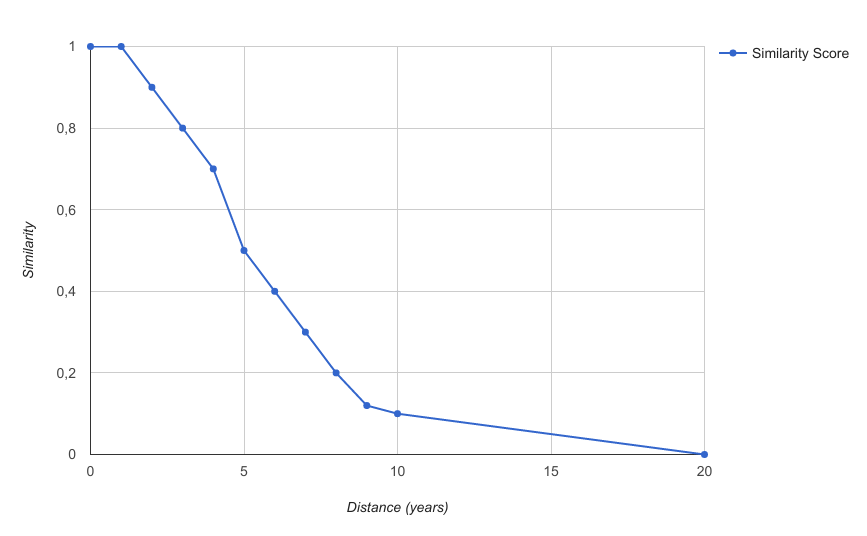
\includegraphics[width=1.0\textwidth]{fig/study_period_graph.png}
    \label{fig:study_period_graph}
\end{figure}

\subsection{Sum Function}

Multi-Criteria Decision Making Methods (MCDMM) are used in myCBR as sum functions by summarizing the similarity score of each attribute in the concept, with regards to the attribute's weight. The myCBR Workbench has two MCDMMs, the Weighted Sum Model (WSM) and the Euclidean Distance. For single dimensional problems, which are the types of problems in the CBR-RS, the WSM can be used without difficulties, and is probably the most common approach \cite{triantaphyllou2000multi} (equation \ref{eq:WSM} \cite{fishburn1967letter}).

\begin{equation} \label{eq:WSM}
    A^{*}_{WSM-score}\quad =\quad max_{i}\  \sum\limits_{j = 1}^{n}\  a_{ij}w_{j},\quad for \quad i =1,\ 2,\ 3,\ ...,\ m.
\end{equation}

When the CBR-RS receives a query, a decision matrix is calculated for each case. This is an $(m \times n)$ matrix where each row is the attribute values of a case, paired with that attributes weight, as shown in Table \ref{tab:decision_matrix}. The WSM is used on this matrix to give each case in the case-base a similarity score between $0-1.0$.


\begin{table}[h]
\centering
\caption{A typical decision matrix for a query from the web application to the CBR-RS}
\label{tab:decision_matrix}
\begin{tabular}{|c|c|c|c|c|c|c|}
 \hline 
Attribute             & $Country$             & $Language$            & \ldots               & \ldots               & \ldots               & $AcademicQuality$     \\\hline 
Weight                & $w_{country}$         & $w_{language}$        & \ldots               & \ldots               & \ldots               & $w_{country}$         \\\hline \hline
$case_{1}$            & $sim_{case_{1}}$      & $sim_{case_{1}}$      & \ldots               & \ldots               & \ldots               & $sim_{case_{1}}$      \\
$case_{2}$            & $sim_{case_{2}}$      & $sim_{case_{2}}$      & \ldots               & \ldots               & \ldots               & $sim_{case_{2}}$      \\
. & . & . & \ldots               & \ldots               & \ldots               & . \\
. & . & . & \ldots               & \ldots               & \ldots               & . \\
. & . & . & \ldots               & \ldots               & \ldots               & . \\
$case_{m}$            & $sim_{case_{m}}$      & $sim_{case_{m}}$      & \ldots               & \ldots               & \ldots               & $sim_{case_{m}}$   \\ \hline 

\end{tabular}
\end{table}


\subsection{Attribute Weights}\label{sec:weighting}

Each attribute in a concept has a value, and an associated weight. This is essentially an integer denoting the importance of that attribute. The results of questionnaire 1, see Table \ref{tab:attribute_ranking}, were used to decide the final weight of the different attributes in the concept, see Table \ref{tab:attribute_weights}.

\begin{table}[h]
\centering
\caption{Finalized weighting of the case attributes}
\label{tab:attribute_weights}
\begin{tabulary}{\textwidth}{|L|R|}
\hline
\textbf{Attribute} & \textbf{Weight} \\ \hline \hline
Home Department & 7.0 \\ \hline
Destination Continent & 2.5 \\ \hline
Destination Country & 4.0 \\ \hline
Destination University & 4.0 \\ \hline
Study Language & 4.0 \\ \hline
Study period & 4.5 \\ \hline
Academic Quality Rating & 3.0 \\ \hline
Social Quality Rating & 3.0 \\ \hline
Ease to find- and quality of residential & 1.5 \\ \hline
Support and reception at university & 2.5 \\ \hline
\end{tabulary}
\end{table}

\FloatBarrier
\section{Test Environment}
The test environment used by Utsida is an essential part of implementation because it was the platform used for the online user test in questionnaire 2. Utsida was hosted on a virtual server provided by Department of Computer Science at NTNU. The virtual server was running Ubuntu 16.04\footnote{Ubuntu, a Debian-based Linux operating system. https://www.ubuntu.com/}. The provided domain name for the prototype was utsida.idi.ntnu.no.

The specific HTTP web server used was Apache2, and it was configured with HTTPS to enable secure and encrypted user sessions. To reduce the effort of running online usability tests and enable users to log in through their university account a service platform using UNINETT's federated authentication service (FEIDE) was implemented. The service platform "Dataporten"\footnote{https://www.uninett.no/en/dataporten} provided by UNINETT enables quick access to important user data and makes possible application users able to log in without registering a user.

Error reporting through email was configured on the server so that alerts were given in case of possible downtime or server errors. Error reporting made it possible to quickly resolve potential bugs or errors on the application and ensure high user satisfaction during the user tests. Tracking user behaviour and statistics could be useful in the final data analysis. Google Analytics was therefore used to increase the understanding of user behaviour. Through Google Analytics it is possible to see a large set of data on the user behaviour. The most important ones used in this project were number of users, average session time, device type and activity flow.  

\cleardoublepage





\iffalse
\paragraph{Completeness} indicates the percentage of stored data versus the total amount of data, which in this case are all the experience reports. Utsida's case-base consists of 8702 cases. However, on The Office of International Relations' website for experience reports, the index goes up to 17012. It is unknown how many reports which are published on this site, because a significant amount of these indexes doesn't point to an experience report, hence, there are a lot less than 17012. Furthermore, many reports were preliminary excluded if they were missing vital information such as which department the student belonged to, or which courses they took on the trip. Without either of this data, a case doesn't give much value to the system. In the end, the cases in the case-base do not represent 100\% completeness with regards to all available experience reports, but they include most of them.

\paragraph{Uniqueness} represents the percentage of data entries which are unique. There is no control regarding duplicate cases in the case-base. Since each case is an individual experience, they are considered unique all though two or more students may have chosen the same geographical place, university, and courses. However, the probability for two cases to be identical is quite slim, as there are so many different attributes and values. Furthermore, in this project, multiple similar cases- even identical ones only strengthen the recommendations for a given query. Other data, such as the assessed course matches, both abroad- and home courses, etc. are required to be unique in Utsida's database, and therefore yields a uniqueness of 100\%.

\paragraph{Timeliness} is the degree to which data represent reality from the required point in time \cite{askham2013six}. The last experience report in the data set was published in 2016, while the first one was published in 1999. The data set should include entries from 2017, but the system for submitting experience reports underwent some changes and updates during fall 2016 and was therefore frozen until spring 2017. This means the newest data in the case-base is already one year older than the current year during the writing of this report (2017). The experience reports tend to be submitted either a couple of months after an exchange period, or in the middle of one. In total, it makes the timeliness have a significant degree of variation and makes it hard to assess. However, even if a student's experience is three years old, it is still likely to be very relevant. Furthermore, the study period attribute is handled in the CBR-RS by reducing a reports relevancy the older it is.

\paragraph{Validity} considers the validity of data, which is valid if it conforms to the syntax (format, type, range) of its definition \cite{askham2013six}. Most of the data in the experience reports were not validated in any way, and free-text was accepted. Because they had no range or constraint, validation had to be done when parsing the reports into cases. The same goes for the assessed course matches.

\paragraph{Accuracy} is the degree to which data correctly describes the \enquote{real world} object or event being described \cite{askham2013six}. Both the data in the experience reports and the assessed course matches is mostly free-text, and thus it was difficult to measure it's accuracy properly. There are no set bounds, ranges and constraints for much of the data, meaning it has to be interpreted. As described in section \ref{sec:parsing_experience_reports}, measures were made to convert data from their free text form to a given format in Utsida, but there are no guarantees for the data ending up as the original user intended.

\paragraph{Consistency} is described as the absence of difference when comparing two or more representations of a thing against a definition \cite{askham2013six}. In the experience reports, this property is considered high. Each report is written in the same exact format, with the same descriptions and values. The assessed course matches, however, lack consistency because the form depends on the student adviser who wrote them. The course matches, therefore, require some analysis and pre-processing before being usable. 

Conclusively, the largest data resource used, the experience reports, is considered to measure poorly in some of the six primary dimensions for data quality assessment. Extensive pre-processing and analysis of the data was essential. All though the methods used may overlook some invalid data, it is considered too small to influence the CBR-RS' recommendations in a noticeable way. 
\fi